\message{ !name(../LuanVanThS_v1.0_main.tex)}\documentclass[a4paper,oneside]{book}
\usepackage[utf8]{vietnam}
\usepackage{amsmath}
\usepackage{amsfonts}
\usepackage{amssymb}
\usepackage{graphicx}
\usepackage{subfig} % gói lệnh cho vẽ nhiều hình trong 1 hình
%\usepackage{subcaption} % gói lệnh cho vẽ nhiều hình trong 1 hình
\usepackage{wrapfig} % gói lệnh vẽ chèn hình vào giữa văn bản
\usepackage{array}  % gói lệnh kẻ bảng với kích thước cố định
\usepackage{tabu}
\usepackage{xcolor}
\usepackage{enumerate} % gói lệnh danh sách
\usepackage[unicode]{hyperref} % gói lệnh tạo liên kết
\usepackage{indentfirst} % Thụt vào đầu mỗi đoạn
\usepackage{pageborder}
\usepackage{comment} %comment khoi lenh
\usepackage{fancybox} 
\usepackage{multirow}
\usepackage{multicol}
\usepackage[left=3.5cm,right=2cm,top=2cm,bottom=2cm]{geometry}
\usepackage{scrextend}
\changefontsizes{13pt} % đặt phông chữ kích thước 13
\linespread{1.2}  % line space multiple 1.2
 \usepackage{fancyhdr}
 \pagestyle{fancy}
 \fancyhf{}
 \usepackage{listings} %Dùng cho định dạng khối lệnh
 \lstset{
 	language=c++, %% Troque para PHP, C, Java, etc... bash é o padrão
 	basicstyle=\ttfamily\small,
 	numberstyle=\footnotesize,
 	% numbers=left,
 	backgroundcolor=\color{gray!10},
 	frame=single,
 	tabsize=2,
 	rulecolor=\color{black!30},
 	title=\lstname,
 	escapeinside={\%*}{*)},
 	breaklines=true,
 	breakatwhitespace=true,
 	framextopmargin=2pt,
 	framexbottommargin=2pt,
 	extendedchars=false,
 	showstringspaces=false,
 	inputencoding=utf8}

\lhead{GVHD: TS. Nguyễn Xuân Hạ}
%\rhead{Luận văn Tốt nghiệp Hệ Cao học Cơ điện tử}

%  \fancyhead[RO]{\rightmark}
\cfoot{\thepage}

\author{Nguyễn Văn Huy}


% ============ BEGIN =================================
\begin{document}

\message{ !name(chapters/chapter12.tex) !offset(-60) }
\chapter{Tổng quan nghiên cứu}
\label{chap:1tqnc}
\section{Giới thiệu robot tự hành}

% - Thế nào là robot tự hành thông minh
% - ứng dụng của robot tự hành thông

%%% Tài liệu tham khảo:
% http://ais.informatik.uni-freiburg.de/teaching/ss18/robotics/ Bài Introduction
% 

Trước đây, nghành robotics tập trung vào nghiên cứu và chế tạo cánh tay robot công nghiệp. Nó được coi như là robot truyền thống (\figurename{\ref{fig:RBCongNghiep}}). Bởi vậy khi nói đến thuật ngữ robot người ta thường nghĩ ngay đến cánh tay robot công nghiệp. \figurename{\ref{fig:RBCongNghiep}} là hình ảnh các cánh tay robot đang làm việc trong khâu sơn khung xe oto. Chúng ta không thấy bóng dáng con người ở trong bức hình này, bởi vì robot công nghiệp truyền thống phải làm việc trong không gian cách ly với con người, có hàng rào bảo vệ vì các lý do an toàn, con người không thể làm việc cùng không gian với robot. 

\begin{figure}[hpt]
  \centering
  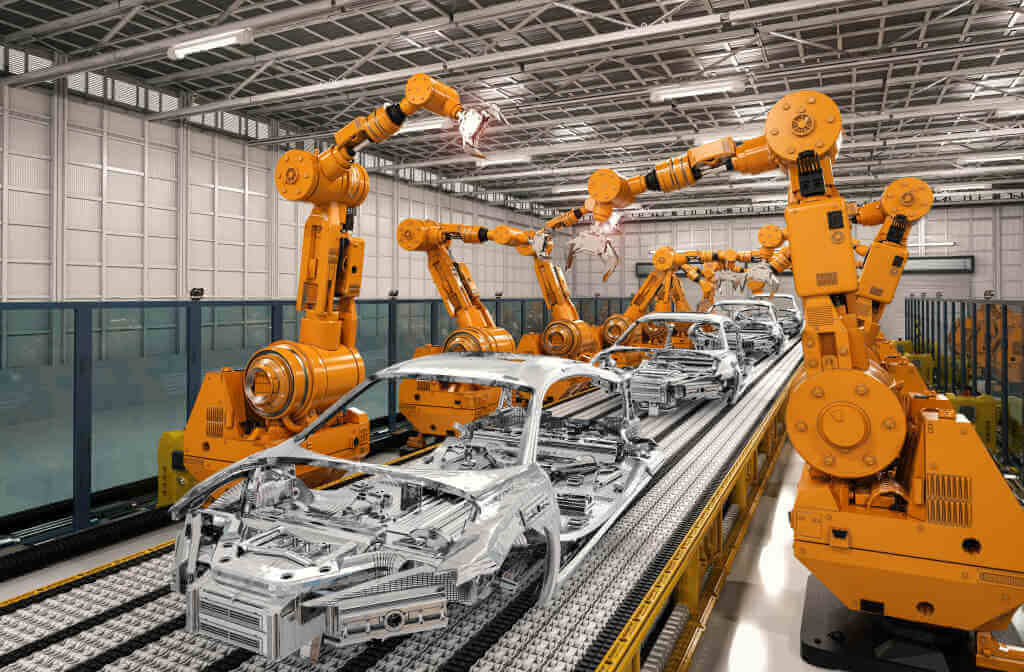
\includegraphics[width=10cm]{figures/IndustrialRobot.jpg}
  \caption{Robot công nghiệp [Nguồn: Internet]}
  \label{fig:RBCongNghiep}
\end{figure}

Bên cạnh đó, robot di động (mobile robot) truyền thống thực hiện các nhiệm vụ di chuyển trên quỹ đạo xác định trước. Robot di động cũng hoạt động dựa trên các khối chương trình được lập trình sẵn. Các phương pháp điều khiển như điều khiển bằng tay thông qua bảng điều khiển, qua sóng RF, wifi... hay di chuyển bám đường chỉ dẫn gắn ở dưới sàn, đọc mã QR, bar. Các phương pháp điều khiển đó đều hạn chế về không gian hoạt động của robot. Việc thiết lập, cấu hình nhà máy, không gian làm việc cho robot hoạt động hết sức tốn kém về chi phí và thời gian mà lại kém linh hoạt.

Ngày nay, robot có xu hướng đi ra khỏi không gian nhà máy, xuất hiện nhiều loại robot như: robot giải trí (\figurename{\ref{fig:rbMoi-a}}), robot dịch vụ cá nhân (\figurename{\ref{fig:rbMoi-b}}) (như máy tính cá nhân), robot trong y tế (\figurename{\ref{fig:rbMoi-c}}); các loại robot tự động trong công nghiệp như robot hái quả (\figurename{\ref{fig:rbMoi-d}}), phun thuốc trong nông nghiệp, robot thông minh tác hợp trong công nghiệp; robot đi tới các môi trường mà con người không tới được như trong lòng đất dưới nước, trên không, trong vũ trụ...
\begin{figure}
	\centering
	\subfloat[][]{
          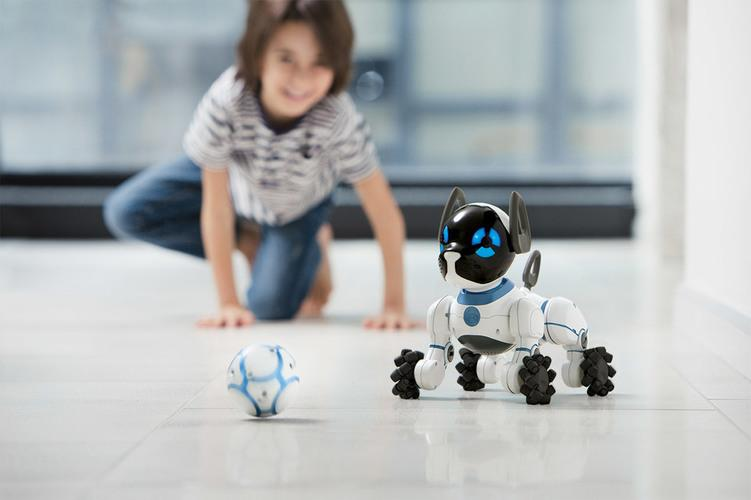
\includegraphics[height=5cm]{figures/c1_entertainmentRobot.jpg}}
          \label{fig:rbMoi-a}
        \subfloat[][]{
          \label{fig:rbMoi-b}
          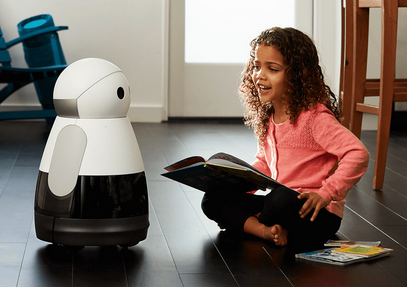
\includegraphics[height=5cm]{figures/c1_personalServiceRobot.png}}
        \hspace{8pt}
        \subfloat[][]{
          \label{fig:rbMoi-c}
          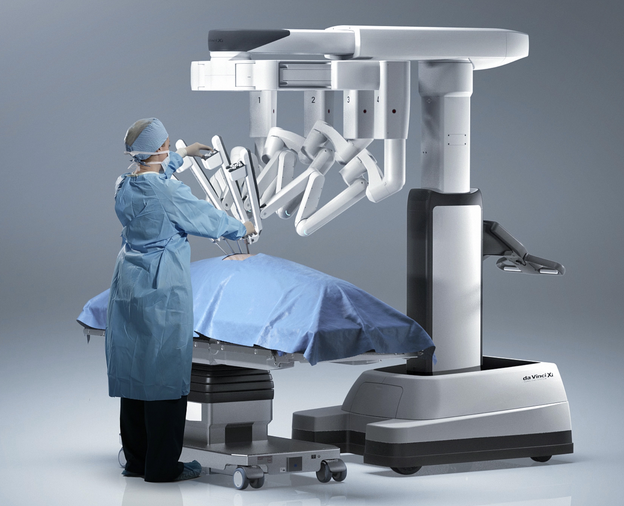
\includegraphics[height=4.6cm]{figures/c1_medicalRobot.png}}
        \subfloat[][]{
          \label{fig:rbMoi-d}
          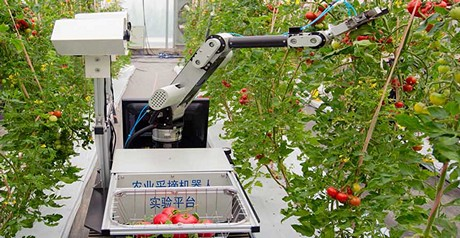
\includegraphics[height=4.6cm]{figures/c1_harvestingRobot.jpg}}
	\hspace{8pt}
	\caption[]{Một số loại robot mới}
	\label{fig:rbMoi}
\end{figure}

\begin{figure}[htp]
  \centering
  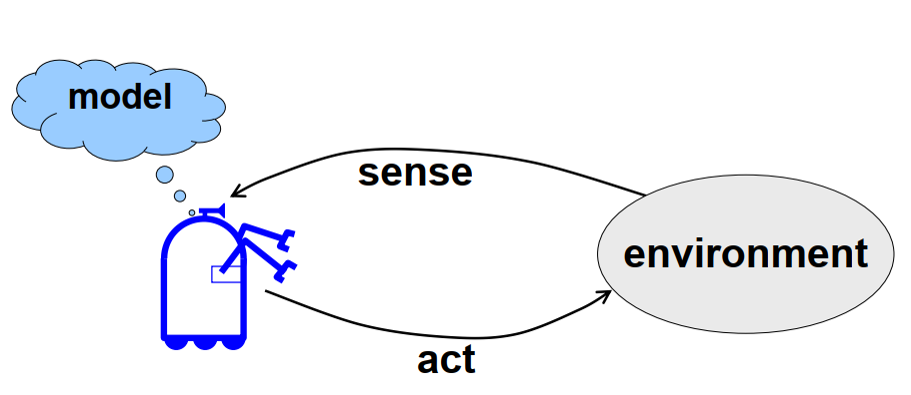
\includegraphics[width=12cm]{figures/c1_AutonomousRBModel.png}
  \caption{Mô hình hệ thống robot tự hành}
  \label{fig:MohinhRB}
\end{figure}

%Trong đó, hệ thống robot tự hành là một dạng robot điển hình cho thế hệ robot mới ngày nay và đang phát triển rất mạnh mẽ. Hệ thống robot tự hành là hệ thống hoạt động như mô hình \figurename{\ref{fig:MohinhRB}}: Robot cảm nhận môi trường thông qua hệ thống cảm biến. Mô hình hóa môi trường sau đó thực hiện các hành động phản ứng lại với môi trường. Các hoạt động cảm nhận môi trường như đo khoảng cách bằng cảm biến siêu âm, hồng ngoại, lidar hay ứng dụng deep learning để nhận dạng đồ vật, người... Các hành động phản ứng có thể là xây dựng bản đồ, thực hiện di chuyển, thực hiện tránh vật, gắp vật...

Robot tự hành thông minh là loại robot di động, có thể cảm nhận, mô hình hóa môi trường xung quanh nó. Thực hiện các hành động di chuyển mà không cần sự giám sát cũng như điều khiển trực tiếp từ con người (\figurename{\ref{fig:MohinhRB}}).

% Có nên thêm phần giới thiệu các robot dựa trên robot tự hành:

\section{Ứng dụng của robot tự hành thông minh}
\label{sec:ungdung}

Với sự thông minh và cực kì linh hoạt của nó, robot tự hành thông minh có rất nhiều ứng dụng. Về cơ bản, nó là nền tảng di chuyển cho tất cả các loại robot di động thông minh ngày nay. Một số sản phẩm ứng dụng trong nhà như:

\begin{itemize}
\item Các ứng dụng trong nhà như robot hút bụi thông minh, robot dịch vụ, robot vận chuyển trong các kho hàng...
\item Các ứng dụng ngoài trời như robot cắt cỏ, chăm sóc cây trồng...
\item Ở các không gian mà con người không tới được như robot thám hiểm dưới nước, trong lòng đất, trên không trung trên các hành tinh khác...
\item Tại các khu vực nguy hiểm như khu vực nhiễm chất phóng xạ, chữa cháy...
\item Và đặc biệt, robot giao hàng tự động, xe tự lái đang phát triển rất nhanh trong những năm gần đây 
\end{itemize}

\section{Các bài toán trên robot tự hành thông minh}

% - Nêu qua concept về điều khiển robot, tạo bản đồ, định vị, path planning, điều hướng, tránh vật cản

\textbf{Cảm biến:} Robot tự hành thông minh cần một số loại cảm biến để có thể hiểu được môi trường, định vị và di chuyển tránh vật cản. 

Có rất nhiều loại cảm biến, để cảm nhận được đa dạng thông tin của môi trường. Có thể chia làm các nhóm như sau:
\begin{itemize}
	\item Khoảng cách 1D: Cảm biến khoảng cách hồng ngoại, siêu âm
	\item Khoảng cách 2D: Lidar
	\item Cảm biến 3D: Có nhiều loại cảm biến 3D như Intel realsense, Microsoft Kinect, Asus Xction...
	\item Ước tính trạng thái robot: GPS, IMU
	\item Cảm biến lực, momen, cảm biến chạm...
	\item Âm thanh, giọng nói như microphone, microphone array
	\item Các loại camera 2D
\end{itemize}

\textbf{Odometry}: là bài toán sử dụng thông tin nhận được từ các cảm biến nhận biết sự di chuyển của robot để ước tính sự thay đổi vị trí của robot qua thời gian. Odometry được sử dụng trong hầu hết các robot tự hành.




\section{Các nghiên cứu tránh vật cản trong robot tự hành thông minh}
\label{sec:tranhVatCan_ref}

% Review các bài báo về tránh vật cản trong robot tự hành
% Chỉ ra các ưu, nhược điểm của các phương pháp như được nêu trong các bài báo trên

\section{Nội dung nghiên cứu}

% Chốt lại nội dung nghiên cứu gồm 2 nội dung:
% - Điều khiển robot ứng dụng SLAM trên nền tảng hệ điều hành ROS
% - Sử dụng Multi-sensor để tăng cường phát hiện và tránh vật cản cho robot
% - Trình bày vắn tắt nội dung của các chương.


%%===========================
\chapter{Cơ sở lý thuyết}
\label{chap:1cslt}
\section{Bài toán về nhiễu trong robot tự hành}

\section{Bài toán SLAM 2D}

\section{Bài toán tạo định vị, tạo bản đồ, điều hướng và tránh vật cản}

\section{Hệ điều hành robot ROS và các ứng dụng}

% Tóm gọn nội dung giới thiệu về ROS và các ứng dụng trong khuôn khổ của luận văn này.

%% ===================
%%% Local Variables:
%%% mode: latex
%%% TeX-master: "../LuanVanThS_v1.0_main"
%%% End:

\message{ !name(../LuanVanThS_v1.0_main.tex) !offset(-96) }

\end{document}

%%% Local Variables:
%%% mode: latex
%%% TeX-master: t
%%% End:
